%%%%%%%%%%%%%%%%%%%%%%%%%%%%%%%%%%%%%%%%%%%%%%%%%%%%%%%%%%%%%%%%%%%%%%%%%%%%%%%%
%%%%%%%%%%%%%%%%%%%%%%%%%%%%%%%%%%%%%%%%%%%%%%%%%%%%%%%%%%%%%%%%%%%%%%%%%%%%%%%%
\section{Percepção rítmica (exercícios)}
\index{Musicalidade!Percepção rítmica}



Como já foi visto na Seção \ref{sec:percepcaosamba1},
existem um conjunto de onomatopeias (``tchic-tchic tum'' e ``tum tum'') que representam tradicionalmente
aos ritmos  que acompanham à melodia principal 
nas músicas que pertencem aos \hyperref[sec:FamiliaSamba]{\textbf{subgêneros do samba}};
estes ritmos de acompanhamento, ou as simplificações que percebemos, 
geralmente tem um padrão muito homogêneo entre compassos sucessivos,
de modo que para um dançarino estes são muito fáceis de predizer 
e podem servir de guia ou como um porto seguro.

Assim, esses ritmos simples geralmente são usados como uma forma que emoldura a execução dos passos básicos 
e alguns mais complexos;
porém, existem passos ou movimentos no samba de gafieira e em outros estilos de dança
que saem desses padrões rítmicos simples. 
\begin{itemize}
\item Em alguns casos,
isto é feito para agregar artisticamente um pouco de complexidade aos movimentos,
porém sem sair-nos completamente da guia do ritmo do acompanhamento; mas 
\item em outros casos, nos saímos dos padrões desse ritmo  
porque deixamos de seguir o ritmo do acompanhamento 
e iniciamos a seguir o ritmo da melodia principal, que geralmente é mais complexa 
e muito heterogênea entre compassos sucessivos\footnote{Este 
tema será abordado mais amplamente na Seção \ref{sec:aspectosusicalidade}.}. 
\end{itemize}


Nesta seção serão presentadas uma serie dinâmicas grupais 
para decorar e acostuma-nos ao uso dos ritmos mais simples e comuns 
a serem achados no acompanhamento do samba de gafieira e outros estilos de dança.

Nestos exemplos está escrito com maiúscula a onomatopeia 
que cai no tempo com acento métrico para lembrar-nos este detalhe na execução do som. 
Também é desenhada uma pauta para descrever os exemplos, 
além de uma representação num diagrama circular 
para facilitar a leitura e execução da pauta.
Nesse diagrama, os círculos pretos representam notas executadas em tempo forte
e os círculos cinza as notas executadas num tempo fraco;
a leitura do diagrama deve ser feito em sentido horário.  

\begin{example}[Treinamentos simples:]
Um professor, ou um software programado, 
deve executar uma ou duas vesses alguma das sequencias rítmicas mostradas nas Figuras 
\ref{fig:abc-percepcionritmica1}, \ref{fig:abc-percepcionritmica2},
\ref{fig:abc-percepcionritmica3}  e \ref{fig:abc-percepcionritmica4}.
Seguidamente os estudantes devem lembrar e repetir o ritmo, 
incluindo as acentuações, dando palmas ou batendo com os pés.
\end{example}


\begin{figure}[H]
\centering
     \begin{subfigure}[c]{0.45\textwidth}
         \centering
         \href{https://drive.google.com/file/d/1c7OawI0qFdiDDiskMlfJAh-l5GYBKVzQ/view?usp=sharing}{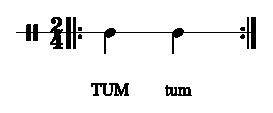
\includegraphics[width=\textwidth]{chapters/cap-musicalidade-percepcion/treino-ritmo1-1.eps}}
         \caption{Pauta do ritmo.}
         \label{fig:RitmoTUMtum1}
     \end{subfigure}
     \hfill
     \begin{subfigure}[c]{0.45\textwidth}
         \centering
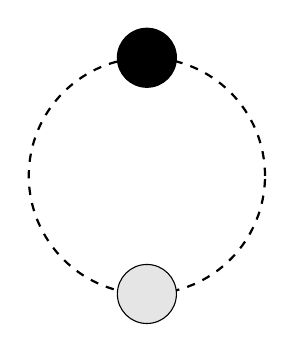
\begin{tikzpicture}
\pgfmathsetmacro{\RadioTot}{1.5}
\pgfmathsetmacro{\Base}{4}
\pgfmathsetmacro{\Radio}{\RadioTot/\Base}
\pgfmathsetmacro{\Theta}{360/\Base}

\draw[black,thick,dashed] (0,0) circle (\RadioTot cm);

\foreach \x in {2}
{
	\draw  [black,fill=gray!20] ({\RadioTot*cos(90-\x*\Theta )} ,{\RadioTot*sin(90-\x*\Theta )})circle (\Radio cm);
}

\foreach \x in {0}
{
	\draw  [black,fill=black] ({\RadioTot*cos(90-\x*\Theta )} ,{\RadioTot*sin(90-\x*\Theta )})circle (\Radio cm);
}
\end{tikzpicture}
         \caption{Diagrama circular do ritmo.}
         \label{fig:RitmoTUMtum2}
     \end{subfigure}
\caption{Descrição do ritmo.}
\label{fig:abc-percepcionritmica1}
\end{figure}


\begin{figure}[H]
\centering
     \begin{subfigure}[c]{0.45\textwidth}
         \centering
         \href{https://drive.google.com/file/d/1Rv5mxppwuJ288xe-EBXf1-5v_tWCvhgc/view?usp=sharing}{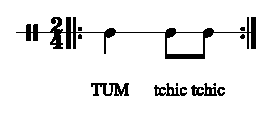
\includegraphics[width=\textwidth]{chapters/cap-musicalidade-percepcion/treino-ritmo2-1.eps}}
         \caption{Pauta do ritmo.}
         \label{fig:RitmoTUMtchictchic1}
     \end{subfigure}
     \hfill
     \begin{subfigure}[c]{0.45\textwidth}
         \centering
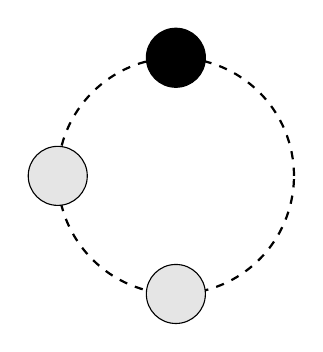
\begin{tikzpicture}
\pgfmathsetmacro{\RadioTot}{1.5}
\pgfmathsetmacro{\Base}{4}
\pgfmathsetmacro{\Radio}{\RadioTot/\Base}
\pgfmathsetmacro{\Theta}{360/\Base}

\draw[black,thick,dashed] (0,0) circle (\RadioTot cm);

\foreach \x in {2,3}
{
	\draw  [black,fill=gray!20] ({\RadioTot*cos(90-\x*\Theta )} ,{\RadioTot*sin(90-\x*\Theta )})circle (\Radio cm);
}

\foreach \x in {0}
{
	\draw  [black,fill=black] ({\RadioTot*cos(90-\x*\Theta )} ,{\RadioTot*sin(90-\x*\Theta )})circle (\Radio cm);
}
\end{tikzpicture}
         \caption{Diagrama circular do ritmo.}
         \label{fig:RitmoTUMtchictchic2}
     \end{subfigure}
\caption{Descrição do ritmo.}
\label{fig:abc-percepcionritmica2}
\end{figure}

\begin{figure}[H]
\centering
     \begin{subfigure}[c]{0.45\textwidth}
         \centering
         \href{https://drive.google.com/file/d/1KJRwnra8i78PsBntrbHOclwRoDMdxtp5/view?usp=sharing}{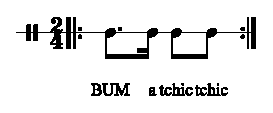
\includegraphics[width=\textwidth]{chapters/cap-musicalidade-percepcion/treino-ritmo3-1.eps}}
         \caption{Pauta do ritmo; $BUM=\frac{3}{4}TUM$.}
         \label{fig:RitmoTUMatchictchic1}
     \end{subfigure}
     \hfill
     \begin{subfigure}[c]{0.45\textwidth}
         \centering
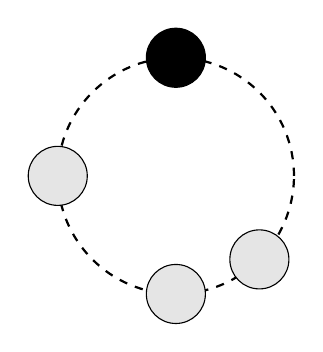
\begin{tikzpicture}
\pgfmathsetmacro{\RadioTot}{1.5}
\pgfmathsetmacro{\Base}{4}
\pgfmathsetmacro{\Radio}{\RadioTot/\Base}
\pgfmathsetmacro{\Theta}{360/\Base}

\draw[black,thick,dashed] (0,0) circle (\RadioTot cm);

\foreach \x in {1.5,2,3}
{
	\draw  [black,fill=gray!20] ({\RadioTot*cos(90-\x*\Theta )} ,{\RadioTot*sin(90-\x*\Theta )})circle (\Radio cm);
}

\foreach \x in {0}
{
	\draw  [black,fill=black] ({\RadioTot*cos(90-\x*\Theta )} ,{\RadioTot*sin(90-\x*\Theta )})circle (\Radio cm);
}
\end{tikzpicture}
         \caption{Diagrama circular do ritmo.}
         \label{fig:RitmoTUMatchictchic2}
     \end{subfigure}
\caption{Descrição do ritmo.}
\label{fig:abc-percepcionritmica3}
\end{figure}


\begin{figure}[H]
\centering
     \begin{subfigure}[c]{0.45\textwidth}
         \centering
         \href{https://drive.google.com/file/d/1ZR0CPhwBYIp2TrqM8cAq_oyI3o-NZPbw/view?usp=sharing}{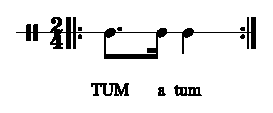
\includegraphics[width=\textwidth]{chapters/cap-musicalidade-percepcion/treino-ritmo4-1.eps}}
         \caption{Pauta do ritmo; $BUM=\frac{3}{4}TUM$}
         \label{fig:RitmoTUMatum1}
     \end{subfigure}
     \hfill
     \begin{subfigure}[c]{0.45\textwidth}
         \centering
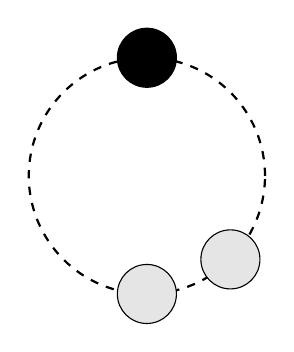
\begin{tikzpicture}
\pgfmathsetmacro{\RadioTot}{1.5}
\pgfmathsetmacro{\Base}{4}
\pgfmathsetmacro{\Radio}{\RadioTot/\Base}
\pgfmathsetmacro{\Theta}{360/\Base}

\draw[black,thick,dashed] (0,0) circle (\RadioTot cm);

\foreach \x in {1.5,2}
{
	\draw  [black,fill=gray!20] ({\RadioTot*cos(90-\x*\Theta )} ,{\RadioTot*sin(90-\x*\Theta )})circle (\Radio cm);
}

\foreach \x in {0}
{
	\draw  [black,fill=black] ({\RadioTot*cos(90-\x*\Theta )} ,{\RadioTot*sin(90-\x*\Theta )})circle (\Radio cm);
}
\end{tikzpicture}
         \caption{Diagrama circular do ritmo.}
         \label{fig:RitmoTUMatum2}
     \end{subfigure}
\caption{Descrição do ritmo.}
\label{fig:abc-percepcionritmica4}
\end{figure}

\begin{example}[Treinamentos elaborados:]
Um professor, ou um software programado, 
deve executar muitas vesses, por exemplo 32, 
as sequencias rítmicas mostradas nas Figuras 
\ref{fig:abc-percepcionritmica5} e \ref{fig:abc-percepcionritmica6}.
Enquanto que os estudantes acompanham o ritmo, 
incluindo as acentuações, dando palmas ou batendo com os pés\footnote{Pode
ser divertido indicar que se pode andar e criar movimentos com os pés, 
sempre que se respeite o ritmo proposto.},
de jeito que a sincronia seja perfeita.
\end{example}

\begin{figure}[H]
\centering
     \begin{subfigure}[c]{0.45\textwidth}
         \centering
         \href{https://drive.google.com/file/d/19gZ2jUqMUFKtJbGxlWl-97hUib1vwEHr/view?usp=sharing}{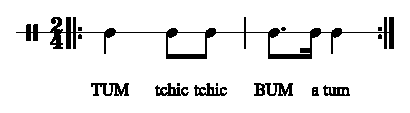
\includegraphics[width=\textwidth]{chapters/cap-musicalidade-percepcion/treino-ritmo5-1.eps}}
         \caption{Pauta do ritmo; $BUM=\frac{3}{4}TUM$}
         \label{fig:Ritmocomplexo1:1}
     \end{subfigure}
     \hfill
     \begin{subfigure}[c]{0.45\textwidth}
         \centering
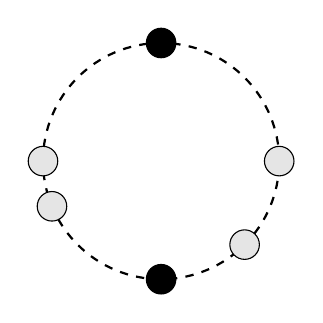
\begin{tikzpicture}
\pgfmathsetmacro{\RadioTot}{1.5}
\pgfmathsetmacro{\Base}{8}
\pgfmathsetmacro{\Radio}{\RadioTot/\Base}
\pgfmathsetmacro{\Theta}{360/\Base}

\draw[black,thick,dashed] (0,0) circle (\RadioTot cm);

\foreach \x in {2,3,5.5,6}
{
	\draw  [black,fill=gray!20] ({\RadioTot*cos(90-\x*\Theta )} ,{\RadioTot*sin(90-\x*\Theta )})circle (\Radio cm);
}

\foreach \x in {0,4}
{
	\draw  [black,fill=black] ({\RadioTot*cos(90-\x*\Theta )} ,{\RadioTot*sin(90-\x*\Theta )})circle (\Radio cm);
}
\end{tikzpicture}
         \caption{Diagrama circular do ritmo.}
         \label{fig:Ritmocomplexo1:2}
     \end{subfigure}
\caption{Descrição do ritmo.}
\label{fig:abc-percepcionritmica5}
\end{figure}





\begin{figure}[H]
\centering
     \begin{subfigure}[c]{0.45\textwidth}
         \centering
         \href{https://drive.google.com/file/d/18Yxz0FwLtXPOD6o5aYRJC10g5i6EZy4E/view?usp=sharing}{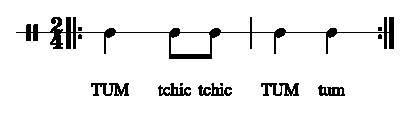
\includegraphics[width=\textwidth]{chapters/cap-musicalidade-percepcion/treino-ritmo6-1.eps}}
         \caption{Pauta do ritmo.}
         \label{fig:Ritmocomplexo2:1}
     \end{subfigure}
     \hfill
     \begin{subfigure}[c]{0.45\textwidth}
         \centering
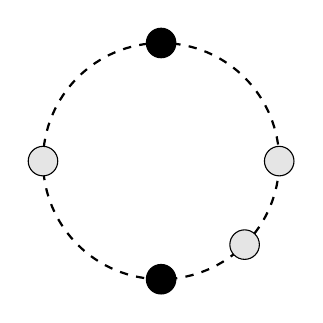
\begin{tikzpicture}
\pgfmathsetmacro{\RadioTot}{1.5}
\pgfmathsetmacro{\Base}{8}
\pgfmathsetmacro{\Radio}{\RadioTot/\Base}
\pgfmathsetmacro{\Theta}{360/\Base}

\draw[black,thick,dashed] (0,0) circle (\RadioTot cm);

\foreach \x in {2,3,6}
{
	\draw  [black,fill=gray!20] ({\RadioTot*cos(90-\x*\Theta )} ,{\RadioTot*sin(90-\x*\Theta )})circle (\Radio cm);
}

\foreach \x in {0,4}
{
	\draw  [black,fill=black] ({\RadioTot*cos(90-\x*\Theta )} ,{\RadioTot*sin(90-\x*\Theta )})circle (\Radio cm);
}
\end{tikzpicture}
         \caption{Diagrama circular do ritmo.}
         \label{fig:Ritmocomplexo2:2}
     \end{subfigure}
\caption{Descrição do ritmo.}
\label{fig:abc-percepcionritmica6}
\end{figure}


\begin{FraseOutros}{Pensamentos aleatórios}{Thomas Sowell} % RANDOM THOUGHTS % Sobre maturidade
Maturidade não é uma questão de idade. Você amadurece quando para de se preocupar em mostrar o quanto é inteligente, e dá total atenção para que dê tudo certo em seu trabalho. Muitos nunca chegam a esse estágio, não importa a idade que tenham  \cite{sowell1999barbarians}.
\end{FraseOutros}

